\documentclass[12pt,a4paper]{article}

\usepackage[spanish]{babel}
\usepackage[utf8]{inputenc}
\usepackage[T1]{fontenc}
\usepackage{lmodern}
\usepackage[a4paper,margin=2.5cm]{geometry}
\usepackage{setspace}
\usepackage{amsmath,amssymb,amsthm}
\usepackage{booktabs}
\usepackage{longtable}
\usepackage{array}
\usepackage{enumitem}
\usepackage{float}
\usepackage{listings}
\usepackage{xcolor}
\usepackage{caption}
\usepackage{graphicx}

% hyperref debe cargarse al final para evitar conflictos
\usepackage[bookmarks=true,bookmarksnumbered=true]{hyperref}

\hypersetup{
    colorlinks=true,
    linkcolor=blue!40!black,
    urlcolor=blue,
    citecolor=black,
    pdftitle={Práctica 2 - Diseño de la red de sensorización},
    pdfauthor={Jan Estrada, Adrian nsq}
}

\setstretch{1.15}
\setlength{\parskip}{0.5em}
\setlength{\parindent}{0pt}

\definecolor{codegray}{rgb}{0.95,0.95,0.95}
\definecolor{codecomment}{rgb}{0.2,0.45,0.2}
\definecolor{codekeyword}{rgb}{0.1,0.1,0.6}

\lstset{
    basicstyle=\ttfamily\small,
    backgroundcolor=\color{codegray},
    frame=single,
    breaklines=true,
    showstringspaces=false,
    commentstyle=\color{codecomment},
    keywordstyle=\color{codekeyword},
    columns=fullflexible
}

\begin{document}

% ---- PORTADA ----
\begin{titlepage}
    \centering
    {\Large \textbf{Optimización}}\\[0.3cm]
    {\large GIA --- UPC}\\[1cm]

    {\huge \textbf{Práctica 2}}\\[0.3cm]
    {\Large Diseño de la red de sensorización para l'Eixample de Barcelona}\\[1.3cm]

    \begin{figure}[H]
        \centering
        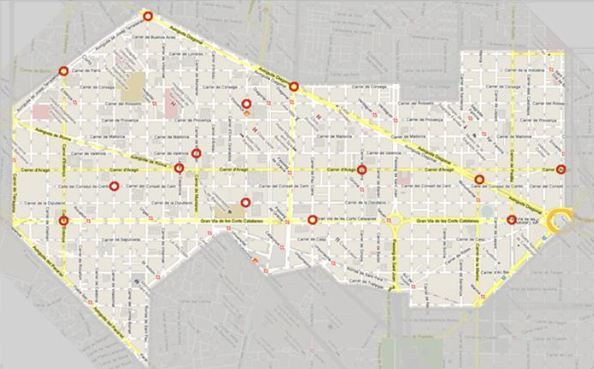
\includegraphics[width=1\linewidth]{image.png}
        \caption{Red de intersecciones de l'Eixample de Barcelona.}
        \label{fig:eixample}
    \end{figure}

    \textbf{Autores}\\[0.3cm]
    Jan Estrada --- DNI: \texttt{26314272H}\\
    Adrian COMPLETAR --- DNI: \texttt{COMPLETAR}\\[1.2cm]

    \textbf{Fecha}\\
    \today\\[2cm]

    \vfill

\end{titlepage}

% ---- ÍNDICE ----
\clearpage
\pdfbookmark[1]{\contentsname}{toc}
\tableofcontents
\clearpage

%% ====================================================================
\section{Introducción}
%% ====================================================================

El problema planteado en esta práctica consiste en diseñar la ubicación óptima de sensores de detección de vehículos en una red urbana de intersecciones del distrito de l'Eixample de Barcelona. El objetivo es maximizar el flujo total de vehículos captado por los sensores, sujeto a un conjunto de restricciones operativas.

En concreto, se pueden instalar como máximo 15 sensores y se debe decidir en qué intersecciones colocarlos. Algunas intersecciones vienen marcadas como \emph{fijas} (el sensor debe colocarse obligatoriamente en ellas) y otras como \emph{prohibidas} (no pueden albergar un sensor bajo ninguna circunstancia). Además, un camino (ruta de vehículos) solo se considera \emph{detectado} si al menos dos de las intersecciones que recorre disponen de un sensor instalado.

Se distinguen dos variantes del problema:

\begin{itemize}
    \item \textbf{Apartado A:} formulación base con el límite de 15 sensores, nodos fijos, nodos prohibidos y detección de caminos.
    \item \textbf{Apartado B:} se añade una restricción técnica adicional que impide que dos sensores se sitúen en intersecciones vecinas, es decir, separadas por una distancia menor o igual a 300 metros.
\end{itemize}

Para resolver ambas variantes se ha seguido un flujo de trabajo en cuatro fases: formulación matemática del modelo como un problema de programación lineal entera binaria (PLEB), preprocesado del fichero de datos original mediante scripts de Python, implementación en lenguaje AMPL y resolución con el solver Gurobi, y finalmente validación e interpretación de los resultados obtenidos.

\subsection{Datos del problema}

Los datos proporcionados por la asignatura incluyen:

\begin{itemize}[itemsep=4pt]
    \item \textbf{457 intersecciones} que conforman la red urbana de l'Eixample.
    \item \textbf{42 caminos} (rutas de vehículos), cada uno con un flujo estrictamente positivo asociado.
    \item \textbf{8 intersecciones fijas} donde el sensor es obligatorio: 30, 78, 44628, 45173, 45481, 45555, 45787 y 49180.
    \item \textbf{3 intersecciones prohibidas} donde no puede haber sensor: 54977, 73703 y 68.
    \item \textbf{542 pares camino--intersección} que definen qué intersecciones forman parte de cada camino.
    \item \textbf{1284 pares de vecindad} (tras normalización) entre intersecciones a 300~m o menos, usados en el apartado B.
\end{itemize}

Un aspecto importante es que de los 15 sensores disponibles, 8 ya vienen fijados de antemano, por lo que el modelo solo decide libremente la ubicación de los 7 sensores restantes. Esto reduce significativamente el espacio de búsqueda, aunque el problema sigue siendo combinatorio.

%% ====================================================================
\section{Organización del proyecto}
%% ====================================================================

Para mantener una estructura clara y separar versiones intermedias de los archivos definitivos, el trabajo se organizó dentro de una carpeta principal \texttt{definitivo/}, subdividida en cuatro bloques funcionales:

\begin{itemize}
    \item \texttt{ampl/}: contiene los modelos \texttt{.mod} (uno por apartado), el fichero de datos \texttt{practica2.dat} y los archivos \texttt{.run} que orquestan la ejecución.
    \item \texttt{tools/}: scripts de Python encargados de parsear el fichero crudo original y generar automáticamente el \texttt{.dat}, así como verificaciones de consistencia previas.
    \item \texttt{datos\_crudos/}: copia íntegra del fichero original entregado por la asignatura, sin modificaciones.
    \item \texttt{notes/}: notas internas de redacción y decisiones consolidadas durante el desarrollo.
\end{itemize}

Esta organización permite separar con claridad el dato original del preprocesado y de la implementación final, y garantiza que el fichero \texttt{.dat} no se ha construido manualmente sino mediante un proceso reproducible.

%% ====================================================================
\section{Formulación matemática}
%% ====================================================================

A continuación se presenta la formulación completa de los dos modelos de programación lineal entera binaria. Se detalla primero el modelo base del apartado A y después la extensión del apartado B.

%% -------------------------------------------------------------------
\subsection{Apartado A --- Modelo base}
%% -------------------------------------------------------------------

\subsubsection{Conjuntos}

\begin{itemize}
    \item $I$: conjunto de todas las intersecciones de la red ($|I| = 457$).
    \item $P$: conjunto de todos los caminos ($|P| = 42$).
    \item $F \subseteq I$: conjunto de intersecciones fijas ($|F| = 8$), donde obligatoriamente debe instalarse un sensor.
    \item $Q \subseteq I$: conjunto de intersecciones prohibidas ($|Q| = 3$), donde no puede situarse ningún sensor.
    \item $I_p \subseteq I$: subconjunto de intersecciones que pertenecen al camino $p \in P$. Este conjunto se materializa en la implementación mediante la relación bidimensional \texttt{PATH\_INTERSECTIONS} $\subseteq P \times I$, que contiene 542 pares.
\end{itemize}

\subsubsection{Parámetros}

\begin{itemize}
    \item $f_p > 0$: flujo de vehículos asociado al camino $p \in P$. El enunciado garantiza que todos los flujos son estrictamente positivos, lo cual es clave para la correcta formulación del modelo (véase la justificación más adelante).
\end{itemize}

\subsubsection{Variables de decisión}

Se utilizan dos familias de variables binarias:

\begin{itemize}
    \item $x_i \in \{0,1\}$, $\forall\, i \in I$: vale 1 si se instala un sensor en la intersección $i$, y 0 en caso contrario.
    \item $y_p \in \{0,1\}$, $\forall\, p \in P$: vale 1 si el camino $p$ se considera detectado, y 0 en caso contrario.
\end{itemize}

La variable $y_p$ es una \textbf{variable auxiliar}: no representa una decisión física (no se ``instala'' nada en un camino), sino que sirve para vincular la presencia de sensores en las intersecciones con el flujo que puede contabilizarse en la función objetivo.

\subsubsection{Función objetivo}

Se desea maximizar el flujo total detectado por los sensores:

\[
\max\; Z = \sum_{p \in P} f_p \, y_p
\]

\subsubsection{Restricciones}

\begin{align}
\sum_{i \in I} x_i &\leq 15 && \text{(límite máximo de sensores)} \label{eq:limit} \\[4pt]
x_i &= 1 \quad \forall\, i \in F && \text{(intersecciones fijas)} \label{eq:fixed} \\[4pt]
x_i &= 0 \quad \forall\, i \in Q && \text{(intersecciones prohibidas)} \label{eq:prohibited} \\[4pt]
\sum_{i \in I_p} x_i &\geq 2\,y_p \quad \forall\, p \in P && \text{(detección de caminos)} \label{eq:detection}
\end{align}

\subsubsection{Justificación de la restricción de detección}

La restricción~\eqref{eq:detection} constituye el núcleo de la modelización y merece una explicación detallada:

\begin{itemize}
    \item \textbf{Si $y_p = 1$} (el camino se marca como detectado), la restricción exige que $\sum_{i \in I_p} x_i \geq 2$, es decir, que al menos dos intersecciones del camino tengan sensor instalado. Esto concuerda exactamente con la definición de camino detectado del enunciado.
    \item \textbf{Si $y_p = 0$} (el camino no se marca como detectado), la restricción se convierte en $\sum_{i \in I_p} x_i \geq 0$, que se satisface trivialmente para cualquier asignación de sensores.
\end{itemize}

Surge entonces la pregunta: ¿no falta una restricción que fuerce $y_p = 1$ cuando un camino \emph{sí} tiene dos o más sensores? La respuesta es \textbf{no}, y la razón es importante: dado que todos los flujos $f_p$ son estrictamente positivos y la función objetivo es de maximización, al solver siempre le interesa activar $y_p = 1$ cuando la restricción~\eqref{eq:detection} lo permite, porque hacerlo incrementa el valor de $Z$. Si un camino tiene dos o más sensores y $y_p$ pudiera valer 1, el solver lo pondrá a 1 por puro interés de maximización. Si no existiera esta garantía (por ejemplo, si algún flujo fuera negativo o nulo), sería necesario añadir una restricción adicional del tipo $y_p \leq \lfloor\sum_{i \in I_p} x_i / 2\rfloor$, complicando innecesariamente el modelo.

\subsubsection{Naturaleza del problema}

El modelo resultante es un problema de \textbf{programación lineal entera binaria} (PLEB o Binary Integer Program, BIP): todas las variables son binarias y todas las restricciones y la función objetivo son lineales. Este tipo de problemas se resuelve mediante algoritmos de ramificación y acotación (branch and bound), que es exactamente lo que realizan solvers como Gurobi o CPLEX.

El tamaño del modelo es moderado: 457 variables $x_i$ + 42 variables $y_p$ = 499 variables binarias, con $1 + 8 + 3 + 42 = 54$ restricciones en el apartado A. Esto permite que los solvers modernos lo resuelvan en fracciones de segundo.

%% -------------------------------------------------------------------
\subsection{Apartado B --- Restricción de separación}
%% -------------------------------------------------------------------

El apartado B reutiliza íntegramente la formulación del apartado A e incorpora una restricción técnica adicional: dos sensores no pueden situarse simultáneamente en intersecciones \emph{vecinas}, definidas como aquellas separadas por una distancia menor o igual a 300 metros.

\subsubsection{Conjunto adicional}

\begin{itemize}
    \item $N \subseteq I \times I$: conjunto de pares de intersecciones vecinas ($|N| = 1284$ pares normalizados).
\end{itemize}

En la implementación, cada par $(i,j)$ se almacena de forma normalizada como $(\min(i,j), \max(i,j))$, lo que elimina duplicados simétricos. Sin esta normalización, el par $(a,b)$ y el par $(b,a)$ generarían dos restricciones idénticas en el modelo, lo cual no causa errores pero sí ineficiencia innecesaria.

\subsubsection{Restricción adicional}

\begin{equation}
x_i + x_j \leq 1 \quad \forall\, (i,j) \in N \label{eq:separation}
\end{equation}

Esta restricción impide que dos sensores queden a una distancia inferior a la mínima permitida. Con ella, el modelo del apartado B tiene $54 + 1284 = 1338$ restricciones, un incremento notable pero que Gurobi sigue resolviendo de forma casi instantánea.

Al añadir la restricción~\eqref{eq:separation}, el conjunto factible del apartado B se reduce respecto al del apartado A: toda solución factible de B también es factible en A, pero no al revés. Formalmente, $\mathcal{F}_B \subseteq \mathcal{F}_A$. Como consecuencia directa:

\[
Z^*_B \leq Z^*_A
\]

es decir, el flujo óptimo del apartado B no puede superar al del A. Si los valores difieren, la diferencia $Z^*_A - Z^*_B$ puede interpretarse como el \textbf{coste} de imponer la restricción de separación mínima entre sensores.

Antes de resolver el apartado B, consideramos que este coste podría ser significativo, dado que 1284 pares de vecindad sobre 457 intersecciones representan una red bastante densa. Sin embargo, como se verá en los resultados, la pérdida fue sorprendentemente pequeña.

%% ====================================================================
\section{Preprocesado en Python}
%% ====================================================================

El fichero original proporcionado por la asignatura (\texttt{OPT25-26\_Datos práctica 2.txt}) no está en un formato directamente utilizable por AMPL. Por ello se desarrollaron dos scripts auxiliares muy sencillos en Python cuyo único propósito es transformar y verificar los datos antes de ejecutar el solver.

\subsection{Parser y generación del \texttt{.dat}}

El script \texttt{tools/build\_ampl\_data.py} implementa un parser directo y minimalista:

\begin{enumerate}
    \item Recorre el fichero crudo línea a línea, detectando cada sección por su cabecera de texto (\texttt{INTERSECTIONS}, \texttt{PATHS}, \texttt{FIXED}, \texttt{PROHIBITED}, \texttt{path\_flow}, \texttt{path\_intersections}, \texttt{intersection\_neighborhood}).
    \item Acumula las líneas de cada sección hasta encontrar la siguiente cabecera.
    \item Genera el fichero \texttt{practica2.dat} con la sintaxis exacta que AMPL espera: conjuntos con \texttt{set ... :=}, parámetros con \texttt{param ... :=}, y conjuntos relacionales con tuplas en formato \texttt{(a, b)}.
    \item Para el conjunto \texttt{NEIGHBORS}, normaliza cada par eliminando vecindades reflexivas (un nodo no es vecino de sí mismo) y duplicados simétricos: \texttt{(min(a,b), max(a,b))}.
\end{enumerate}

Al terminar, el script imprime un resumen de cardinalidades que usamos como comprobación de coherencia:

\begin{lstlisting}[caption={Salida del parser}]
Intersections: 457
Paths: 42
Path intersections: 542
Neighbors: 1284
\end{lstlisting}

Se optó por un parser sencillo en lugar de uno más complejo con validaciones exhaustivas, ya que el formato del fichero crudo es regular y predecible. Cualquier inconsistencia en los datos (referencias a intersecciones inexistentes, flujos negativos, etc.) será detectada inmediatamente por AMPL durante la carga del \texttt{.dat}, gracias a las declaraciones \texttt{within} y \texttt{> 0} del modelo.

\subsection{Verificación de conflictos entre nodos fijos}

El script \texttt{tools/verify\_fixed\_intersections.py} realiza una comprobación específica previa al apartado B: recorre la lista de nodos \texttt{FIXED} y la estructura de vecindad para detectar si existen dos nodos fijos que además sean vecinos entre sí.

¿Por qué es necesaria esta verificación? Si existieran dos nodos fijos vecinos, el modelo del apartado B sería \textbf{intrínsecamente infactible}:
\begin{itemize}
    \item La restricción~\eqref{eq:fixed} obligaría a instalar sensor en ambos: $x_i = x_j = 1$.
    \item La restricción~\eqref{eq:separation} lo prohibiría: $x_i + x_j \leq 1$.
    \item Ambas restricciones serían mutuamente excluyentes, haciendo el problema irresoluble.
\end{itemize}

Este tipo de infactibilidad es difícil de diagnosticar a posteriori a partir del mensaje del solver, por lo que conviene detectarla \emph{antes} de lanzar la ejecución. La comprobación es rápida (unas pocas líneas de código) y ahorra potenciales dolores de cabeza.

La ejecución del script confirmó que \textbf{no existen conflictos} entre nodos fijos vecinos, por lo que procedimos con confianza a resolver el modelo del apartado B.

%% ====================================================================
\section{Implementación en AMPL}
%% ====================================================================

\subsection{Elección del solver}

Se utilizó \textbf{Gurobi 13.0.0} como solver para ambos apartados. Gurobi es un solver comercial de alto rendimiento para problemas de programación lineal, entera y mixta, ampliamente utilizado tanto en ámbitos académicos como industriales. Se eligió sobre otras alternativas (como CPLEX o los solvers open-source) por estar disponible localmente en la instalación de AMPL del equipo de trabajo y por ofrecer garantía de optimalidad global para problemas de este tipo.

Al tratarse de un problema de tamaño moderado (499 variables binarias, entre 54 y 1338 restricciones), cualquier solver MILP competente habría sido adecuado. De hecho, los tiempos de resolución fueron prácticamente instantáneos en ambos casos.

\subsection{Fichero de datos unificado}

Una decisión de diseño importante fue utilizar un \textbf{único fichero} \texttt{practica2.dat} para ambos apartados, en lugar de uno por modelo. Este fichero contiene todos los conjuntos y parámetros, incluido \texttt{NEIGHBORS}.

En el modelo del apartado A, el conjunto \texttt{NEIGHBORS} se declara pero no se utiliza en ninguna restricción:

\begin{lstlisting}
# Declarado para compartir practica2.dat con el apartado B.
set NEIGHBORS within {INTERSECTIONS, INTERSECTIONS};
\end{lstlisting}

AMPL requiere que todo conjunto presente en el fichero \texttt{.dat} esté declarado en el \texttt{.mod}, aunque no participe en ninguna restricción. Esta declaración ``vacía'' es inocua y evita tener que mantener dos ficheros de datos distintos, lo cual sería propenso a errores de sincronización.

\subsection{Modelo del apartado A (\texttt{practica2\_a.mod})}

La implementación sigue fielmente la formulación matemática:

\begin{lstlisting}[caption={Modelo AMPL completo del apartado A}]
set INTERSECTIONS;
set PATHS;
set FIXED within INTERSECTIONS;
set PROHIBITED within INTERSECTIONS;
set PATH_INTERSECTIONS within {PATHS, INTERSECTIONS};
# Declarado para compartir practica2.dat con el apartado B.
set NEIGHBORS within {INTERSECTIONS, INTERSECTIONS};

param PATH_FLOW {PATHS} > 0;

var x {i in INTERSECTIONS} binary;
var y {p in PATHS} binary;

maximize total_flow:
    sum {p in PATHS} PATH_FLOW[p] * y[p];

subject to sensor_budget:
    sum {i in INTERSECTIONS} x[i] <= 15;

subject to detected_paths {p in PATHS}:
    sum {(p, i) in PATH_INTERSECTIONS} x[i] >= 2 * y[p];

subject to fixed_sensors {i in FIXED}:
    x[i] = 1;

subject to prohibited_sensors {i in PROHIBITED}:
    x[i] = 0;
\end{lstlisting}

Algunos aspectos relevantes de la implementación:

\begin{itemize}[itemsep=4pt]
    \item La declaración \texttt{PATH\_FLOW \{PATHS\} > 0} impone positividad estricta del flujo. Si algún camino tuviera flujo nulo o negativo en el \texttt{.dat}, AMPL rechazaría los datos antes de resolver, evitando resultados incorrectos.
    \item La restricción \texttt{detected\_paths} utiliza la notación \texttt{(p, i) in PATH\_INTERSECTIONS} para iterar únicamente sobre los pares camino--intersección que realmente existen (542 pares), lo que es mucho más eficiente que un indexado completo sobre $P \times I$ (que serían $42 \times 457 = 19194$ combinaciones).
    \item Las declaraciones \texttt{within INTERSECTIONS} en \texttt{FIXED} y \texttt{PROHIBITED} actúan como comprobación de integridad referencial: si el \texttt{.dat} contuviera un nodo fijo que no existiera en \texttt{INTERSECTIONS}, AMPL daría error inmediatamente.
\end{itemize}

\subsection{Modelo del apartado B (\texttt{practica2\_b.mod})}

El modelo del apartado B es idéntico al del apartado A, con la adición de una única familia de restricciones:

\begin{lstlisting}[caption={Restricción adicional en el apartado B}]
subject to separated_sensors {(i, j) in NEIGHBORS}:
    x[i] + x[j] <= 1;
\end{lstlisting}

Dado que el conjunto \texttt{NEIGHBORS} está normalizado (cada par aparece una sola vez como $(\min,\max)$), no se generan restricciones duplicadas.

\subsection{Ficheros \texttt{.run}}

Los ficheros \texttt{.run} orquestan la ejecución completa: cargan el modelo y los datos, seleccionan el solver y muestran los resultados. Ambos tienen la misma estructura:

\begin{lstlisting}[caption={Fichero \texttt{practica2\_a.run} (análogo para el apartado B)}]
model practica2_a.mod;
data practica2.dat;
option solver gurobi;
solve;
display total_flow;
display {i in INTERSECTIONS : x[i] = 1} x[i];
display {p in PATHS : y[p] = 1} y[p];
\end{lstlisting}

Se ha optado por mostrar únicamente las variables activas (con valor 1) mediante la condición \texttt{x[i] = 1} en el \texttt{display}. Esto produce una salida limpia y legible, en lugar de listar las 457 intersecciones con sus valores (casi todos 0).

%% ====================================================================
\section{Resultados}
%% ====================================================================

Ambos modelos se resolvieron localmente con \textbf{Gurobi 13.0.0} a través de la interfaz de AMPL. Los dos alcanzaron el estado \texttt{optimal solution}, lo que garantiza que las soluciones reportadas son \textbf{globalmente óptimas}: no existe ninguna otra asignación de sensores que produzca un flujo mayor.

\subsection{Resumen general}

\begin{table}[H]
\centering
\caption{Resumen comparativo de resultados}
\begin{tabular}{>{\raggedright\arraybackslash}p{5cm}cc}
\toprule
\textbf{Magnitud} & \textbf{Apartado A} & \textbf{Apartado B} \\
\midrule
Estado del solver          & Óptimo             & Óptimo \\
Flujo total detectado      & 350,734            & 350,178 \\
Número de sensores         & 15                 & 15 \\
Caminos detectados         & 24                 & 24 \\
Iteraciones símplex        & 43                 & 75 \\
Nodos de ramificación      & 1                  & 1 \\
Solver                     & Gurobi 13.0.0      & Gurobi 13.0.0 \\
\bottomrule
\end{tabular}
\end{table}

El flujo total detectado del apartado A ($Z^*_A = 350{,}734$) es ligeramente superior al del apartado B ($Z^*_B = 350{,}178$), tal como se esperaba al tratarse de un conjunto factible más restrictivo. La diferencia es:

\[
\Delta Z = Z^*_A - Z^*_B = 350{,}734 - 350{,}178 = 0{,}556
\]

Este resultado fue sorprendente: dado que el apartado B añade 1284 restricciones de vecindad, esperábamos una pérdida de flujo más significativa. Sin embargo, la diferencia es de apenas un $0{,}16\%$ del total. Esto sugiere que la topología de l'Eixample es lo suficientemente amplia como para que los sensores puedan redistribuirse sin una gran penalización.

Otro dato notable es que ambos apartados requirieron \textbf{solo 1 nodo de ramificación} en el algoritmo branch-and-bound. Esto indica que la relajación lineal del problema (es decir, el mismo modelo pero con variables continuas en $[0,1]$ en vez de binarias) produce una solución muy cercana a la entera, y Gurobi apenas necesita explorar el árbol de soluciones. Es un indicador de que el modelo está bien formulado y es ``fácil'' desde el punto de vista computacional.

\subsection{Sensores seleccionados}

\begin{table}[H]
\centering
\caption{Intersecciones con sensor en cada apartado (15 nodos)}
\begin{tabular}{>{\raggedright\arraybackslash}p{2.5cm} p{10cm}}
\toprule
\textbf{Apartado} & \textbf{Intersecciones con sensor ($x_i = 1$)} \\
\midrule
A & 5, 30, 78, 20349, 41633, 41970, 44494, 44609, 44628, 45173, 45481, 45555, 45787, 49180, 54839 \\[4pt]
B & 5, 30, 78, 41633, 41653, 41970, 44522, 44609, 44628, 45173, 45481, 45555, 45787, 49180, 54839 \\
\bottomrule
\end{tabular}
\end{table}

\subsubsection{Análisis comparativo de los sensores}

Ambas soluciones comparten \textbf{13 de los 15 sensores}:

\begin{itemize}[itemsep=4pt]
    \item Los \textbf{8 nodos fijos} (30, 78, 44628, 45173, 45481, 45555, 45787, 49180) aparecen en ambas soluciones, como imponen las restricciones.
    \item Los nodos \textbf{5, 41633, 41970, 44609} y \textbf{54839} se seleccionan libremente en ambos apartados. El hecho de que estos 5 nodos sean elegidos en las dos variantes indica que son intersecciones muy rentables: participan en muchos caminos de alto flujo y no entran en conflicto con ninguna restricción de vecindad.
\end{itemize}

Las diferencias se concentran en dos nodos:

\begin{itemize}[itemsep=4pt]
    \item \textbf{Apartado A} incluye los nodos \textbf{20349} y \textbf{44494}, que no aparecen en B.
    \item \textbf{Apartado B} incluye los nodos \textbf{41653} y \textbf{44522} como sustitutos.
\end{itemize}

Estos cambios se deben a que la restricción de separación~\eqref{eq:separation} invalida la combinación de nodos 20349 y/o 44494 con algún otro nodo seleccionado (por ser vecinos a menos de 300~m), forzando al solver a buscar las siguientes mejores alternativas. Es interesante notar que el solver no simplemente ``elimina'' dos nodos y deja huecos, sino que reemplaza por otros nodos que permiten seguir detectando un número igual de caminos (24 en ambos casos).

\subsection{Caminos detectados}

\begin{table}[H]
\centering
\caption{Caminos detectados ($y_p = 1$) en cada apartado}
\begin{tabular}{>{\raggedright\arraybackslash}p{2.5cm} p{10cm}}
\toprule
\textbf{Apartado} & \textbf{Caminos detectados} \\
\midrule
A (24 caminos) & 1439, 1441, 1451, 1479, 1483, 1484, 1488, 1492, 1493, 1499, 1500, 1504, 1513, 1516, 1518, 1536, 1537, 1541, 1547, 1549, 1550, 1560, 1561, 1577 \\[4pt]
B (24 caminos) & 1445, 1451, 1479, 1483, 1484, 1488, 1492, 1493, 1499, 1500, 1504, 1513, 1516, 1518, 1525, 1536, 1537, 1541, 1547, 1549, 1550, 1560, 1561, 1577 \\
\bottomrule
\end{tabular}
\end{table}

Ambas soluciones detectan \textbf{24 de 42 caminos}, pero con ligeras diferencias en cuáles se detectan:
\begin{itemize}
    \item El apartado A detecta los caminos \textbf{1439} ($f = 3{,}019$) y \textbf{1441} ($f = 0{,}202$), que no aparecen en B.
    \item El apartado B detecta los caminos \textbf{1445} ($f = 0{,}088$) y \textbf{1525} ($f = 2{,}577$), que no aparecen en A.
\end{itemize}

Esto es coherente con los cambios de sensores: al reubicar los nodos con sensor, cambian los caminos que cumplen la condición de tener al menos dos intersecciones sensorizadas. La diferencia neta de flujo es:
\[
(3{,}019 + 0{,}202) - (0{,}088 + 2{,}577) = 3{,}221 - 2{,}665 = 0{,}556
\]
que coincide exactamente con $\Delta Z$ calculado antes, lo cual sirve como comprobación cruzada de coherencia.

\subsection{Dominancia del camino 1513}

Un aspecto muy destacable es que el camino \textbf{1513} tiene un flujo de $f_{1513} = 261{,}109$ vehículos, que representa por sí solo aproximadamente el \textbf{74,5\%} del flujo total detectado. Este camino pasa por solo 6 intersecciones (44604, 44609, 44616, 44623, 44628, 44635), dos de las cuales (44609 y 44628) son seleccionadas como sensor en ambos apartados (44628 es un nodo fijo). Esto significa que la sola presencia de estos dos sensores justifica la mayor parte del valor objetivo.

El resto de los 23 caminos detectados aportan conjuntamente los $\approx 89{,}6$ unidades restantes, con contribuciones individuales mucho más modestas.

%% ====================================================================
\section{Verificación de coherencia}
%% ====================================================================

Para confirmar la validez de los resultados, se verificaron los siguientes criterios de coherencia sobre ambas soluciones:

\begin{itemize}[itemsep=6pt]
    \item \textbf{Nodos fijos:} los 8 sensores fijos (30, 78, 44628, 45173, 45481, 45555, 45787, 49180) aparecen activados ($x_i = 1$) en ambas soluciones. $\checkmark$
    \item \textbf{Nodos prohibidos:} los 3 nodos prohibidos (54977, 73703, 68) no aparecen entre los sensores seleccionados en ningún apartado. $\checkmark$
    \item \textbf{Límite de sensores:} ambas soluciones instalan exactamente 15 sensores. $\checkmark$
    \item \textbf{Optimalidad:} Gurobi reporta \texttt{optimal solution} en ambos casos, con gap de MIP nulo en el apartado B (\texttt{absmipgap = 5.68e-14}, esencialmente cero). $\checkmark$
    \item \textbf{Relación $Z^*_B \leq Z^*_A$:} se cumple ($350{,}178 \leq 350{,}734$), confirmando la relación teórica entre los conjuntos factibles. $\checkmark$
    \item \textbf{Coherencia cruzada de flujos:} la diferencia $\Delta Z = 0{,}556$ coincide exactamente con la suma de flujos de los caminos ganados y perdidos entre A y B, como se calculó anteriormente. $\checkmark$
    \item \textbf{Separación en apartado B:} se comprobó visualmente que ningún par de nodos seleccionados en B aparece en el conjunto \texttt{NEIGHBORS}. $\checkmark$
\end{itemize}

%% ====================================================================
\section{Conclusiones}
%% ====================================================================

La resolución de esta práctica se ha abordado mediante una formulación de programación lineal entera binaria clara y compacta, implementada de forma directa en AMPL y resuelta con Gurobi 13.0.0. El preprocesado previo en Python, aunque sencillo e intencionadamente minimalista, ha sido útil para:

\begin{enumerate}[itemsep=4pt]
    \item Evitar errores de transcripción manual en un fichero de datos con 457 intersecciones, 42 caminos, 542 pares camino--intersección y 1284 relaciones de vecindad.
    \item Verificar la consistencia del dataset antes de ejecutar el solver, descartando infactibilidades estructurales (conflictos entre nodos fijos vecinos en el apartado B).
    \item Generar un fichero \texttt{.dat} unificado, reutilizable por ambos modelos sin duplicar información.
\end{enumerate}

Los resultados obtenidos permiten extraer las siguientes conclusiones:

\begin{itemize}[itemsep=4pt]
    \item Ambos modelos son factibles y alcanzan el óptimo global, con tiempos de resolución prácticamente instantáneos.
    \item La restricción de separación del apartado B tiene un impacto operativo muy reducido ($\Delta Z \approx 0{,}16\%$). Esto sugiere que la topología de l'Eixample, con su estructura reticular regular, permite distribuir los sensores eficientemente incluso respetando la distancia mínima de 300~m.
    \item La solución está fuertemente dominada por el camino 1513, cuyo flujo ($261{,}109$) representa el 74,5\% del total detectado. Esto implica que la decisión más crítica es asegurar que este camino quede detectado, lo cual ocurre en ambos apartados.
    \item El hecho de que ambas soluciones utilicen los 15 sensores indica que la restricción es activa: con más sensores disponibles, podrían detectarse caminos adicionales.
    \item Los 5 nodos elegidos libremente que coinciden en ambos apartados (5, 41633, 41970, 44609, 54839) representan intersecciones de importancia estratégica en la red, al participar en múltiples caminos de alto flujo.
\end{itemize}

En una aplicación real sería imprescindible asegurar que las restricciones técnicas se cumplen exactamente como se han modelado, especialmente la distancia mínima entre sensores. Además, cabría estudiar la sensibilidad del modelo a variaciones en los flujos o en el número máximo de sensores, para evaluar la robustez de la solución ante cambios en las condiciones operativas.

\end{document}
